%\chapter{det-comp}


%%%%%%%%%%%%%%%%%%%%%%%%%%%%%%%%%%%%%%%%%%%%%%
%\section{Anode Plane Assemblies}

%%%%%%%%%%%%%%%%%%%%%%%%%%%%%%%%%%%%%%%%%%%%%%
%\section{Cathode Plane Assemblies}

%%%%%%%%%%%%%%%%%%%%%%%%%%%%%%%%%%%%%%%%%%%%%%
\section{Field Cage}

%%%%%%%%%%%%%%%%%%%%%%%%%
\subsection{Scope, Requirements and Design Parameters}

\fixme{I added a bit of explanation that isn't in earlier sections yet (Anne)}
In the ProtoDUNE-SP TPC, 
the six APAs are arranged into two APA planes, each consisting of three side-by-side APAs. Between them,  
%, flanking either side of 
a central cathode plane splits the TPC volume into two
electron-drift regions, one between
each pair of facing cathode and anode planes. %forms an electron-drift region. 
A field cage (FC) must completely surround the four
open sides of the entire drift %this 
region %to provide the necessary boundary conditions
to ensure that the %a uniform
 electric field within is uniform and unaffected by the presence
of the cryostat walls and other nearby conductive structures.

\fixme{Adding a bit from docdb 1504; would be nice to include its fig 6.1; need orig, not one copied from Word doc.  }
\fixme{One field cage with many assemblies or modules? Clarify assembly vs module} 

The ProtoDUNE-SP TPC will have six top and six bottom field cage assemblies, arranged three across each horizontal edge of the two drift regions. It will have 
four endwall panels, one at each vertical edge of the two drift regions.
Each endwall panel consists of four assemblies in ``landscape'' orientation, stacked vertically.
FC assemblies are constructed from pultruded G10 I-beams and box beams that support extruded field-shaping aluminum profiles. The support structure for each of the top and bottom FC assemblies consists of two main I-beams that are 3.6~m long, and four cross I-beams \fixme{length?} that connect the main I-beams for structural stability.


The main I-beams have cutouts to hold the field-shaping profiles. Main I-beams are spliced at 2.5~m to facilitate drift distance %change of the TPC from 3.6 m to 
of 2.5~m. Splice joints and cross I-beam joints are held together using an arrangement of shear pins and plates. 

Aside from the profiles themselves, the nuts and bolts holding them, and the ground planes, all FC components are made of insulating material. The material selected for these structural components is fiberglass-reinforced plastic (FRP), which will prevent binding when the structure is at cryogenic temperatures. The ground planes are made of stainless steel. 

\fixme{from docdb 1504 sec 6.3 I can't tell if there's ONE ground plane at the TOP, ONE at the BOTTOM or two. In this section it appears plural. 1504 needs clarification. }

The bottom face \fixme{on the bottom, isn't it the top face? Should we say inward-facing face?} of the ground planes will be approximately 20~cm away from the top of the field-shaping profiles. The ground planes are mounted at a fixed distance from the field shaping profiles by using standoffs, as shown in Figure 6.2 \fixme{reference properly}, which shows ground planes over I-beams and cross beams.

%The ProtoDUNE-SP field cages are constructed from tiled field cage modules.  
%Each FC module is built with a number of 
The parallel metal profiles in a FC module 
\fixme{assembly?} are interconnected by a resistive divider chain, and supported by the FRP beams that span the drift volume between the CPA and one of the APAs. 
The metal profiles between modules are neither mechanically nor electrically connected. The electrical isolation between the field cage modules minimizes the peak energy dump in case of a HV discharge.

\fixme{The above needs work!}

\begin{cdrfigure}[The field cages]{fc-overview}{A view of the TPC field cage}
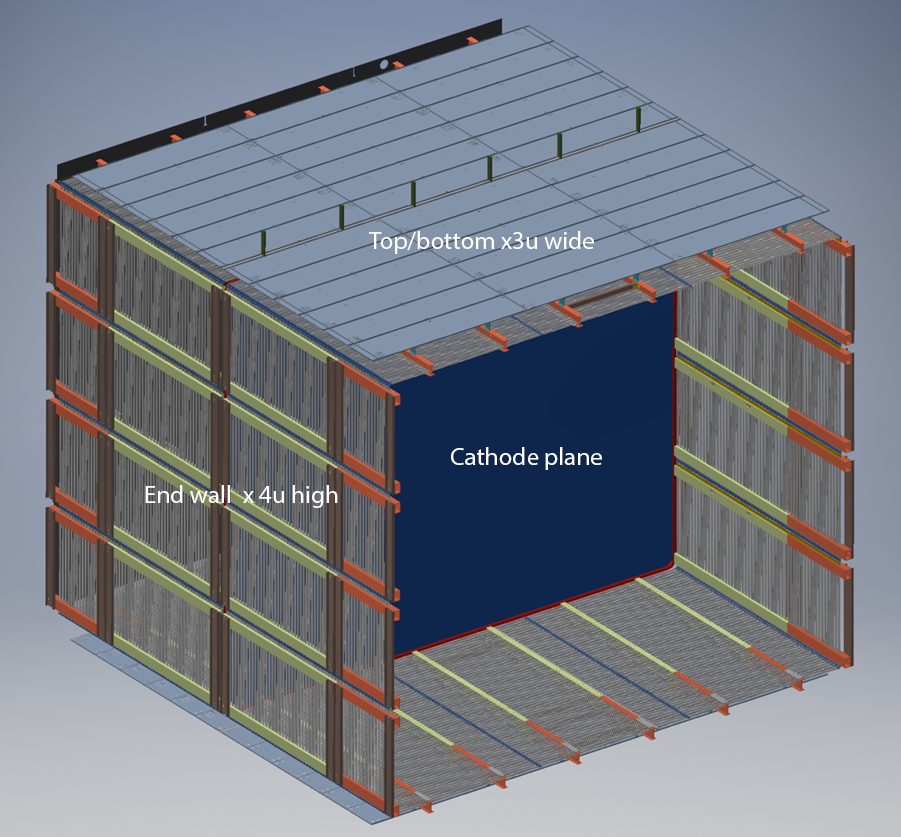
\includegraphics[width=0.8\linewidth]{tpc_fc_overview.png}
\end{cdrfigure}
\fixme{Figure~\ref{fc-overview} is not referenced. It also needs a fuller, more descriptive caption}

The FC is required to:
\begin{itemize}
\item provide the nominal drift field of 500V/cm;
\item withstand $-$180kV near the cathode;
\item define the drift distance between the APAs and CPAs to <1~cm;
\item limit the electric field %exposed to LAr 
in the LAr volume to under 30~kV/cm;
\item miminize the peak energy transfer in case of a HV discharge anywhere on the field cage or cathode;
\item provide redundancy in the resistor divider; \fixme{this feels incomplete... ``in the resistor-divider chain?}
\item maintain the divider current %must be >> 
much greater than the ionization current in the TPC drift cell, yet less than the power supply current limit when all dividers are connected in parallel;
\item %Constructed in 
be modular in form such that they can be easily installed in the cryostat;
\item provide support for the beam plug;
\item allow calibration laser beams to enter into the active volume; 
\item support a 200-lb. person standing on the support beam of the bottom field cage module;
\item be configurable to either 3.6~m or 2.5~m drift length inside the cryostat; and
\item %No 
prevent any trapped volume.

\end{itemize}

%%%%%%%%%%%%%%%%%%%%%%%%%
\subsection{Electrical Design}

Given a large standoff distance between the field cage and the grounded cryostat wall, it is relatively easy to design a field cage that meets the 30-kV/cm E field limit with 180-kV bias.  However, It becomes challenging %if we want 
to reduce the clearance between the FC and ground in order to make more efficient use of liquid argon.  %To achieve this goal, one must look for 
This requires an electrode with a low profile, rounded edges, no trapped volume, and low cost.  Several commercially available roll-formed metal profiles were studied and appear to meet these requirements. \fixme{what's challenging about it then?}


%%%%%%%%%%%%
\subsubsection{Electrostatic analysis}

%One particular profile (
The Dahlstrom Roll Form \#1071 was found to have the lowest surface E field, which was about 12~kV/cm when biased at 180~kV with only a 20-cm ground clearance (see Figure~\ref{fig:fc-profile1071}).

\begin{cdrfigure}[2D FEA of roll formed profiles]{fc-profile1071}{A 2D FEA of a configuration using profile 1071, and a conceptual design of the field cage module}
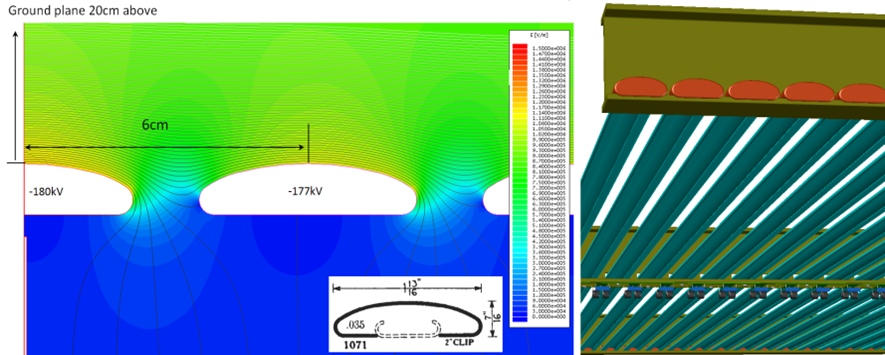
\includegraphics[width=0.8\linewidth]{tpc_fc_profile1071.png}
\end{cdrfigure}
  
In order to maintain a modular design of the field cage while minimizing peak energy transfer in a discharge,% we chose to construct 
the field cage will be constructed with electrical isolation between neighboring modules. %such that 
If a discharge occurs on one field cage, the %nearby 
electrodes from the neighboring modules will not arc over and cause a domino effect.  This requires a %high (I found `high voltage' here confusing)
voltage insulation between profile ends of the order of 180~kV.  UHMW PE caps of 5-mm thickness are placed over both ends of each profile to serve this purpose. This technique also limits the exposed electric field in LAr at the corner of the field cage, see Figure~\ref{fig:fc_corner}. \fixme{What's the deal with ``exposed'' E field in LAr? The E field exists in the LAr; I don't understand what ``exposure'' refers to here}

\begin{cdrfigure}[3D FEA of field cage corner]{fc_profile_corner}{A 3D FEA of a field cage corner.  The PE caps (in outline form) limit the exposed E field to}
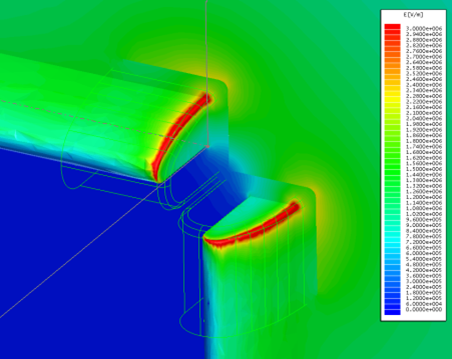
\includegraphics[width=0.6\linewidth]{tpc_fc_profile_corner.png}
\end{cdrfigure}

The center-to-center distance between the profiles is set to 6~cm, and the inner surface of all profiles on a field cage module is placed 5~cm beyond the nearest surface of the TPC active volume (defined by the APA active aperture over the drift distance). The E field uniformity at the edge of the active volume is expected to be within $\pm$2\% of the nominal value.


%%%%%%%%%%%%  
\subsubsection{Surge suppressor on field cage}

The resistors along the divider provide a linear DC voltage gradient. However, at shorter time scales ($\ll$1~s), the electrical behavior of the divider is determined by the various capacitances on and between each electrode, and %.  This divider
 is no longer linear at this time scale. 

A perfect capacitive divider requires the capacitance of each node to ground to be zero.  In reality, there is always a finite capacitance from each node to ground, and these capacitances resist change in the voltages on the nodes. In the event of a HV breakdown between the cathode %to 
and ground (cryostat), the cathode voltage quickly collapses to ground, but the first FC electrode-to-ground capacitance keeps its voltage from changing instantaneously to follow the cathode voltage, resulting in a momentarily larger voltage differential between the cathode and the first FC electrode. This voltage differential can be a significant fraction of the cathode operating voltage, large enough to cause HV breakdown between the two electrodes, or worse yet, to destroy the divider resistors between the two electrodes.

A natural solution to this problem is to significantly increase the capacitance between the nodes of this divider. This was the approach adopted in the 35-ton prototype's field cage through the use of double-sided printed circuit boards (PCB).  However, the cost of the PCB version of the field cage at DUNE scale is very high, and adding discrete HV capactitors between divider taps is also expensitive.

An alternative is to use surge surpressors in parallel with the divider resistors to divert the transient current from the resistors. Extensive tests have been done by MicroBooNE (docdb 3242, arXiv:1406.5216v2) \fixme{add in bib and cite here} on the use of metal oxide varistors (MOVs) and gas discharge tubes (GDTs) as a means of limiting the over-voltage condition in the event of a HV discharge in the TPC. 

Both types will work for the purpose of restricting the voltage differential between field cage rings in LAr temperature. 
A GDT quickly shorts the terminals when the voltage differential exceeds a threshold, while
a varistor changes its resistance to keep the voltage differential near the threshold voltage.
The smooth transition and well defined clamping voltage of the varistors are preferred to the abrupt switching of the GDTs.
The varistors could also function as redundant ``resistors'' in a divider chain in case a resistor is open circuit. \fixme{open circuited?}

One readily available MOV famility \fixme{family?} with high threshold voltage is the Panasonic ERZ-VXXD182.  These have a threshold voltage around 1600~V.  Two of these in series could work with the current 3-kV differential between divider taps.  However, this configuration would not allow raising the E field much above the nominal 500~V/cm.  To allow some headroom in operating field, three such MOVs in series would be needed.


%%%%%%%%%%%%
\subsubsection{Resister tolerance and specification}

\begin{cdrfigure}[The resistive divider]{fc-divider-view}{A view of a resistive divider}
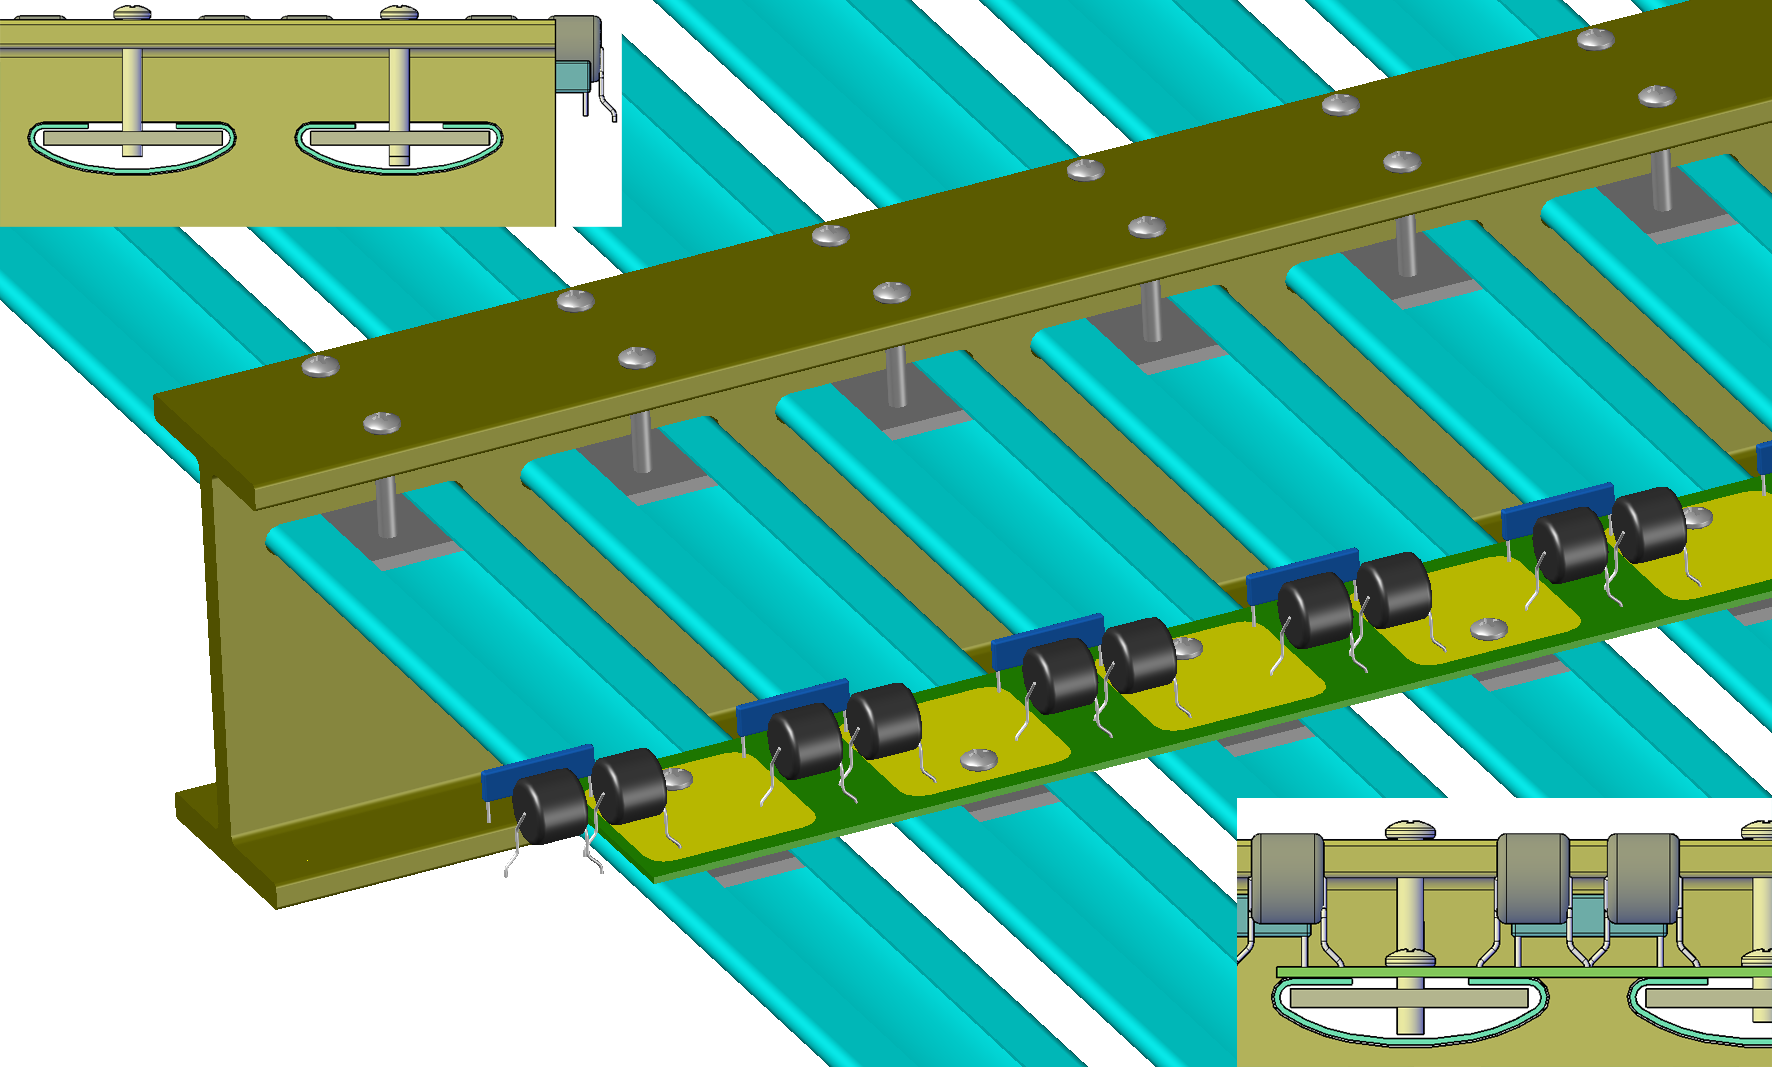
\includegraphics[width=0.8\linewidth]{tpc_fc_r_divider.png}
\end{cdrfigure}

%%%%%%%%%%%%
\subsubsection{Electrical schematic}
 
\begin{cdrfigure}[Field cage schematic diagram]{fc-schematic}{A schematic diagram of the CPA and a top/bottom field cage module pair}
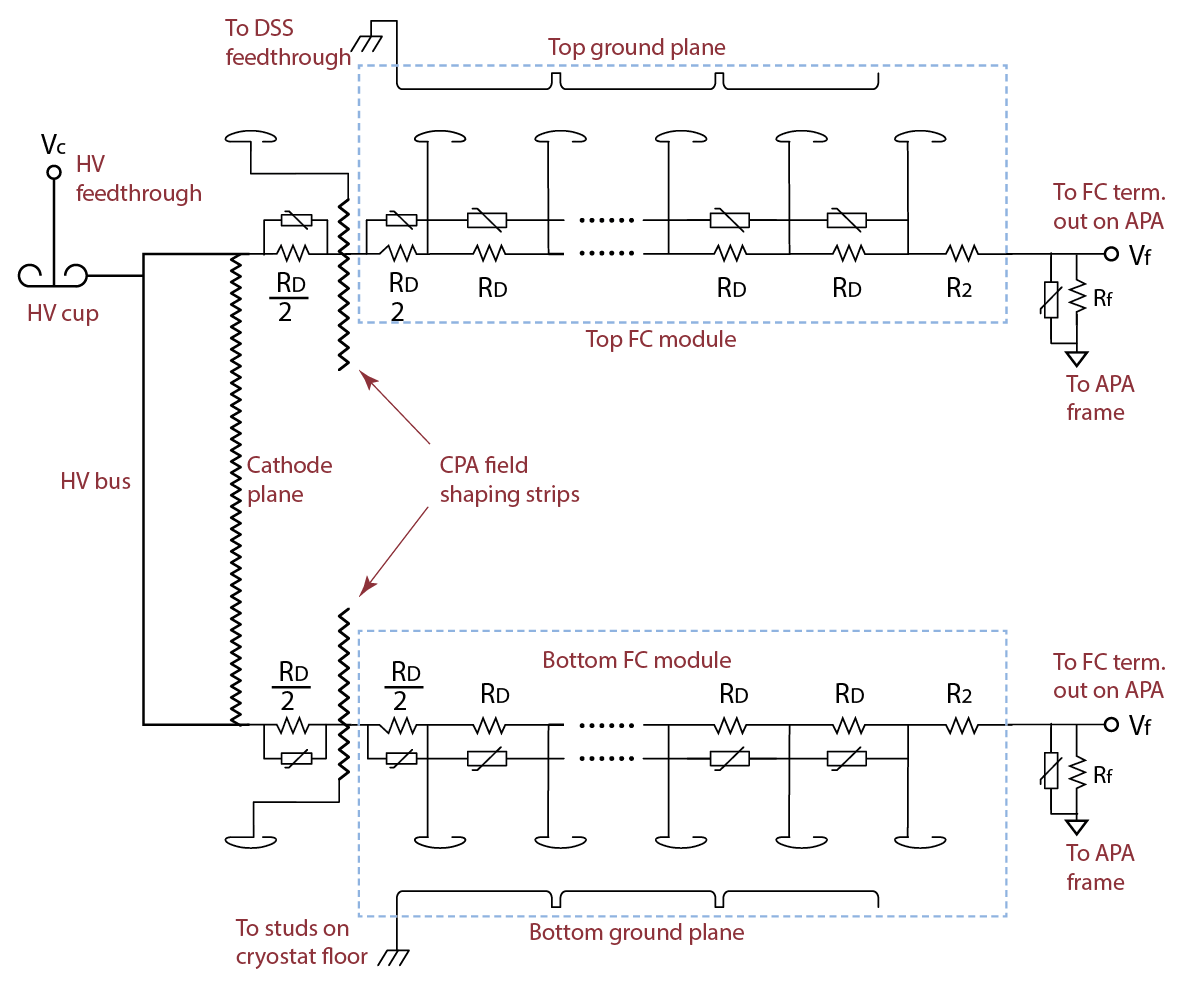
\includegraphics[width=0.8\linewidth]{tpc_fc_schematic.png}
\end{cdrfigure}

%%%%%%%%%%%%%%%%%%%%%%%%%
\subsection{Validation tests of roll-formed FC design}

A dedicated test setup has been designed and constructed to validate the field cage concept  in purified LAr.
It consists of a field cage (Figure~\ref{fig:fc-test}), fitting into the ICARUS 50-liter cryostat (1.1~m hight, 0.6~m diameter) available at CERN, and  includes:

\begin{itemize}	
\item roll-formed metal profiles with UHMW PE caps,
\item pultruded fiberglass I-beams form four mini panels,
\item HV cable feed-through (equipped with corona monitor) allowing application of up to 150~kV on FC profiles,
\item all profiles at same potential to simplify HV connection,
\item ICARUS-like stainless steel ground planes placed  66~mm away from FC profiles ($\sim$1/3 of FD bias voltage to reach
same E field), and
\item video cameras in the gas phase to monitor bubbles and sparks.
\end{itemize}

\begin{cdrfigure}[The field cage test setup]{fc-test}{The field cage test setup. 
 {\bf Left:} schematic drawings of the cage showing the main elements: metal profiles, I-beams, ground planes.
  {\bf Right:} Picture of the realized setup.}
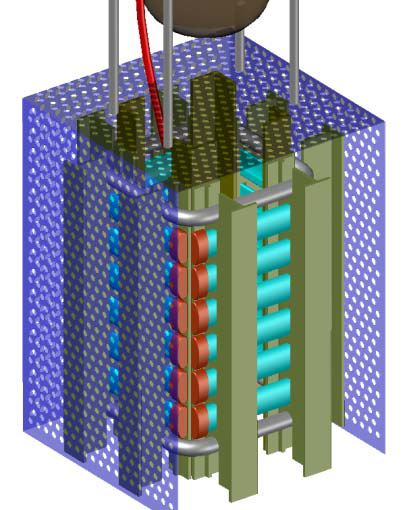
\includegraphics[width=0.45\linewidth]{tpc_fc-test-1.png}
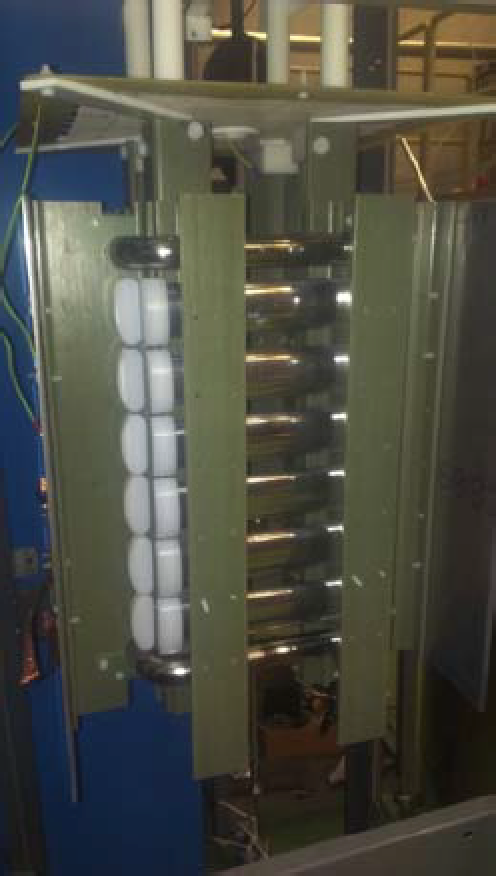
\includegraphics[width=0.45\linewidth]{tpc_fc-test-2.png}
\end{cdrfigure}

Two choices of material (aluminum, stainless steel) for the metal profiles have been tested. In the aluminum case, the surface finish has also been tested with scratches up to 100 microns deep. 

The cage was operated both in commercial LAr and, connected to the ICARUS 50-liter recirculation system, in LAr with purity  better that 0.1 ppb O$_2$ equivalent. HV above 80~kV (corresponding to an electric field about 20\% higher than nominal) could be 
\fixme{was?} applied for several days, without recording any discharge. Two additional regimes have been studied:
\begin{itemize}	
\item  With the 50-liter vessel fully thermalized (no visible bubble formation along the detector), no sparks appear %(were ever recorded) 
with voltage up to 100~kV.
\item  HV instabilities arise in the 80$-$100 kV range if the LAr is not perfectly thermalized, allowing bubble formation from heat sources (HV feedthrough, ground connections): a few random sparks were recorded, developing however around the HV cable and not between the field cage and the ground plates.
\end{itemize}

All tested materials exhibited the same behavior in the applied HV range. 

Nickel coating (up to 20 microns) of aluminum profiles was also proposed as a way to avoid oxidation of the surface, which % could possibly be 
is a potential source of HV instability. Its stability against  thermal gradients was positively tested. \fixme{tested and found to be positive, i.e, stable? Pls clarify} However HV tests showed no difference with respect to the uncoated version.

A specific breakdown test has been performed to check dielectric rigidity of the UHMW PE end caps in LAr. %exposing a few metal profiles equipped with PE end caps and connected the HV, to a ground plane (Figure~\ref{fig:endcap-test}).
A few metal profiles equipped with PE end caps and connected the HV were exposed to a ground plane (Figure~\ref{fig:endcap-test}).
Results demonstrated that the proposed end-cap geometry and thickness can safely hold 150~kV.

\begin{cdrfigure}[Setup to test dielectric rigidity]{endcap-test}{Setup to test dielectric rigidity of the UHMW PE end caps}
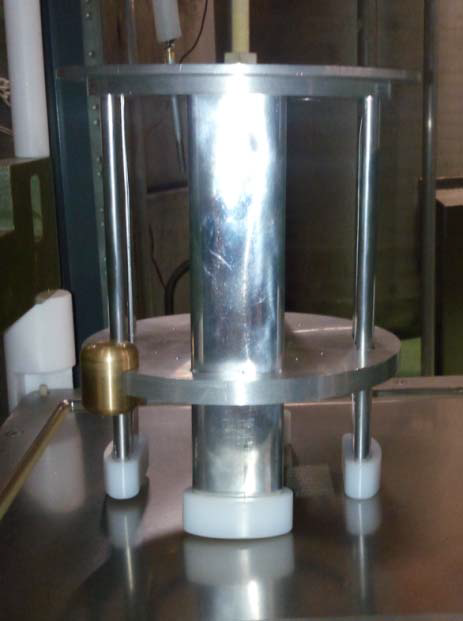
\includegraphics[width=0.65\linewidth]{tpc_fc_endcap-test.png}
\end{cdrfigure}

%%%%%%%%%%%%%%%%%%%%%%%%%
\subsection{Ground Plane Design}
%% by A. Zani

In order to confine the electric field in the liquid argon region, it is foreseen to install a metallic plane, put to ground, 
\fixme{``a grounded metallic plane''?}
between the upper field cage module and the liquid-gas interface. The design of such a Ground Plane (GP) \fixme{need to define acronym above and just use it} is inspired by the one from the ICARUS T600 detector, and it is meant to limit the residual electric field in the liquid below the usual 30~kV/cm value. 
\fixme{Is it to keep the E field from going outside the LAr volume or is it to keep the residual field that's already in the LAr volume very small?}
%The design details of the planes were verified to comply with the requests on residual electric field with FEA.  It is noted that a similar GP could be added in front of all the other Field Cage (FC) modules, in order to smooth the field in the LAr dead volume. However, so far it is foreseen to add an actual GP only below the bottom FC, to further smooth the field in the region where pipings for the cryostat filling are running. The distance between the cryostat walls and the end-wall field cage does not require to insert a GP, instead.
The design details of the planes were verified for compliance with the requests on residual electric field with FEA. \fixme{I cannot parse prev sentence} It is noted that a similar GP could be added in front of each of the other Field Cage (FC) modules in order to smooth the field in the LAr dead volume. However, so far it is planned to add one only below the bottom FC, to further smooth the field in the region where pipings for the cryostat filling  run. The distance between the cryostat walls and the end-wall field cage does not require insertion of a GP.

As mentioned, the GP design is inspired by the ICARUS T600 detector: in that case, 1 mm thick Stainless Steel (SS) plates, punched with $10$ mm holes, 15 mm pitch ($\sim 50\%$ transparency), could stand a potential differential of $-150$ kV over $100$ mm. In order to smooth the field, the edges of the planes were rounded to $\sim 10$ mm. The fraction of punched structure was selected to ensure light-weight even with SS, and to allow fluid circulation above the planes.

\fixme{Does this mean: This GP is similar to the one in the ICARUS detector, (the listed features are the same for both). The ICARUS GP can withstand a potential differential of $-150$ kV over $100$ mm, therefore ours can, too.  In  ICARUS, the edges of the GPs were rounded to $\sim 10$ mm, so we plan to do the same?  Is our punched fraction different than ICARUS's because we want it to be lighter-weight or allow more fluid flow? }

In the ProtoDUNE-SP configuration, the GP will be put at a distance of 200~mm from the FC profile, with a structure of $6$ mm holes, $10$ mm pitch ($\sim 25\%$ transparency): the lower fraction of pierced surface is verified by simulations to maintain the field within the required values. The edges of the plates, $20$ mm high, are rounded at $5$ mm, while the holes rounding radius, at production is around $0.5$ mm. The liquid level is expected to be at 40 mm above the GP bottom, i.e. 20 mm above the edges. The radius of curvature for the holes is not a strict requirement. It depends on the punching technique, and usually is at around $0.5$ mm. The actual requirement is to have the hole curvature on the inside (of the TPC) looking out.
\fixme{The previous pgraph needs clarification}

Two sets of pieces \fixme{two sets of GPs? Define ``piece''} were initially produced in Europe:
\begin{itemize}
\item 8 pieces of dimension $198 \times 571$ mm (weight $< 1$ kg each) to be installed in the CERN field cage prototype,
\item 6 more pieces of  $525 \times 2318$ mm (weight around $8.5$ kg each), which represent full scale components for ProtoDUNE-SP. The drawing of this second set of pieces, sent to the U.S. for test assemblies, in shown in Figure~\ref{fig:gp_panels}.
\end{itemize}

\begin{cdrfigure}[ProtoDUNE GP]{gp_panels}{Top: Techincal Drawing, by Claudio Montanari, of the Ground Plane panels for ProdoDUNE-SP. Bottom: 3D model of one panel}
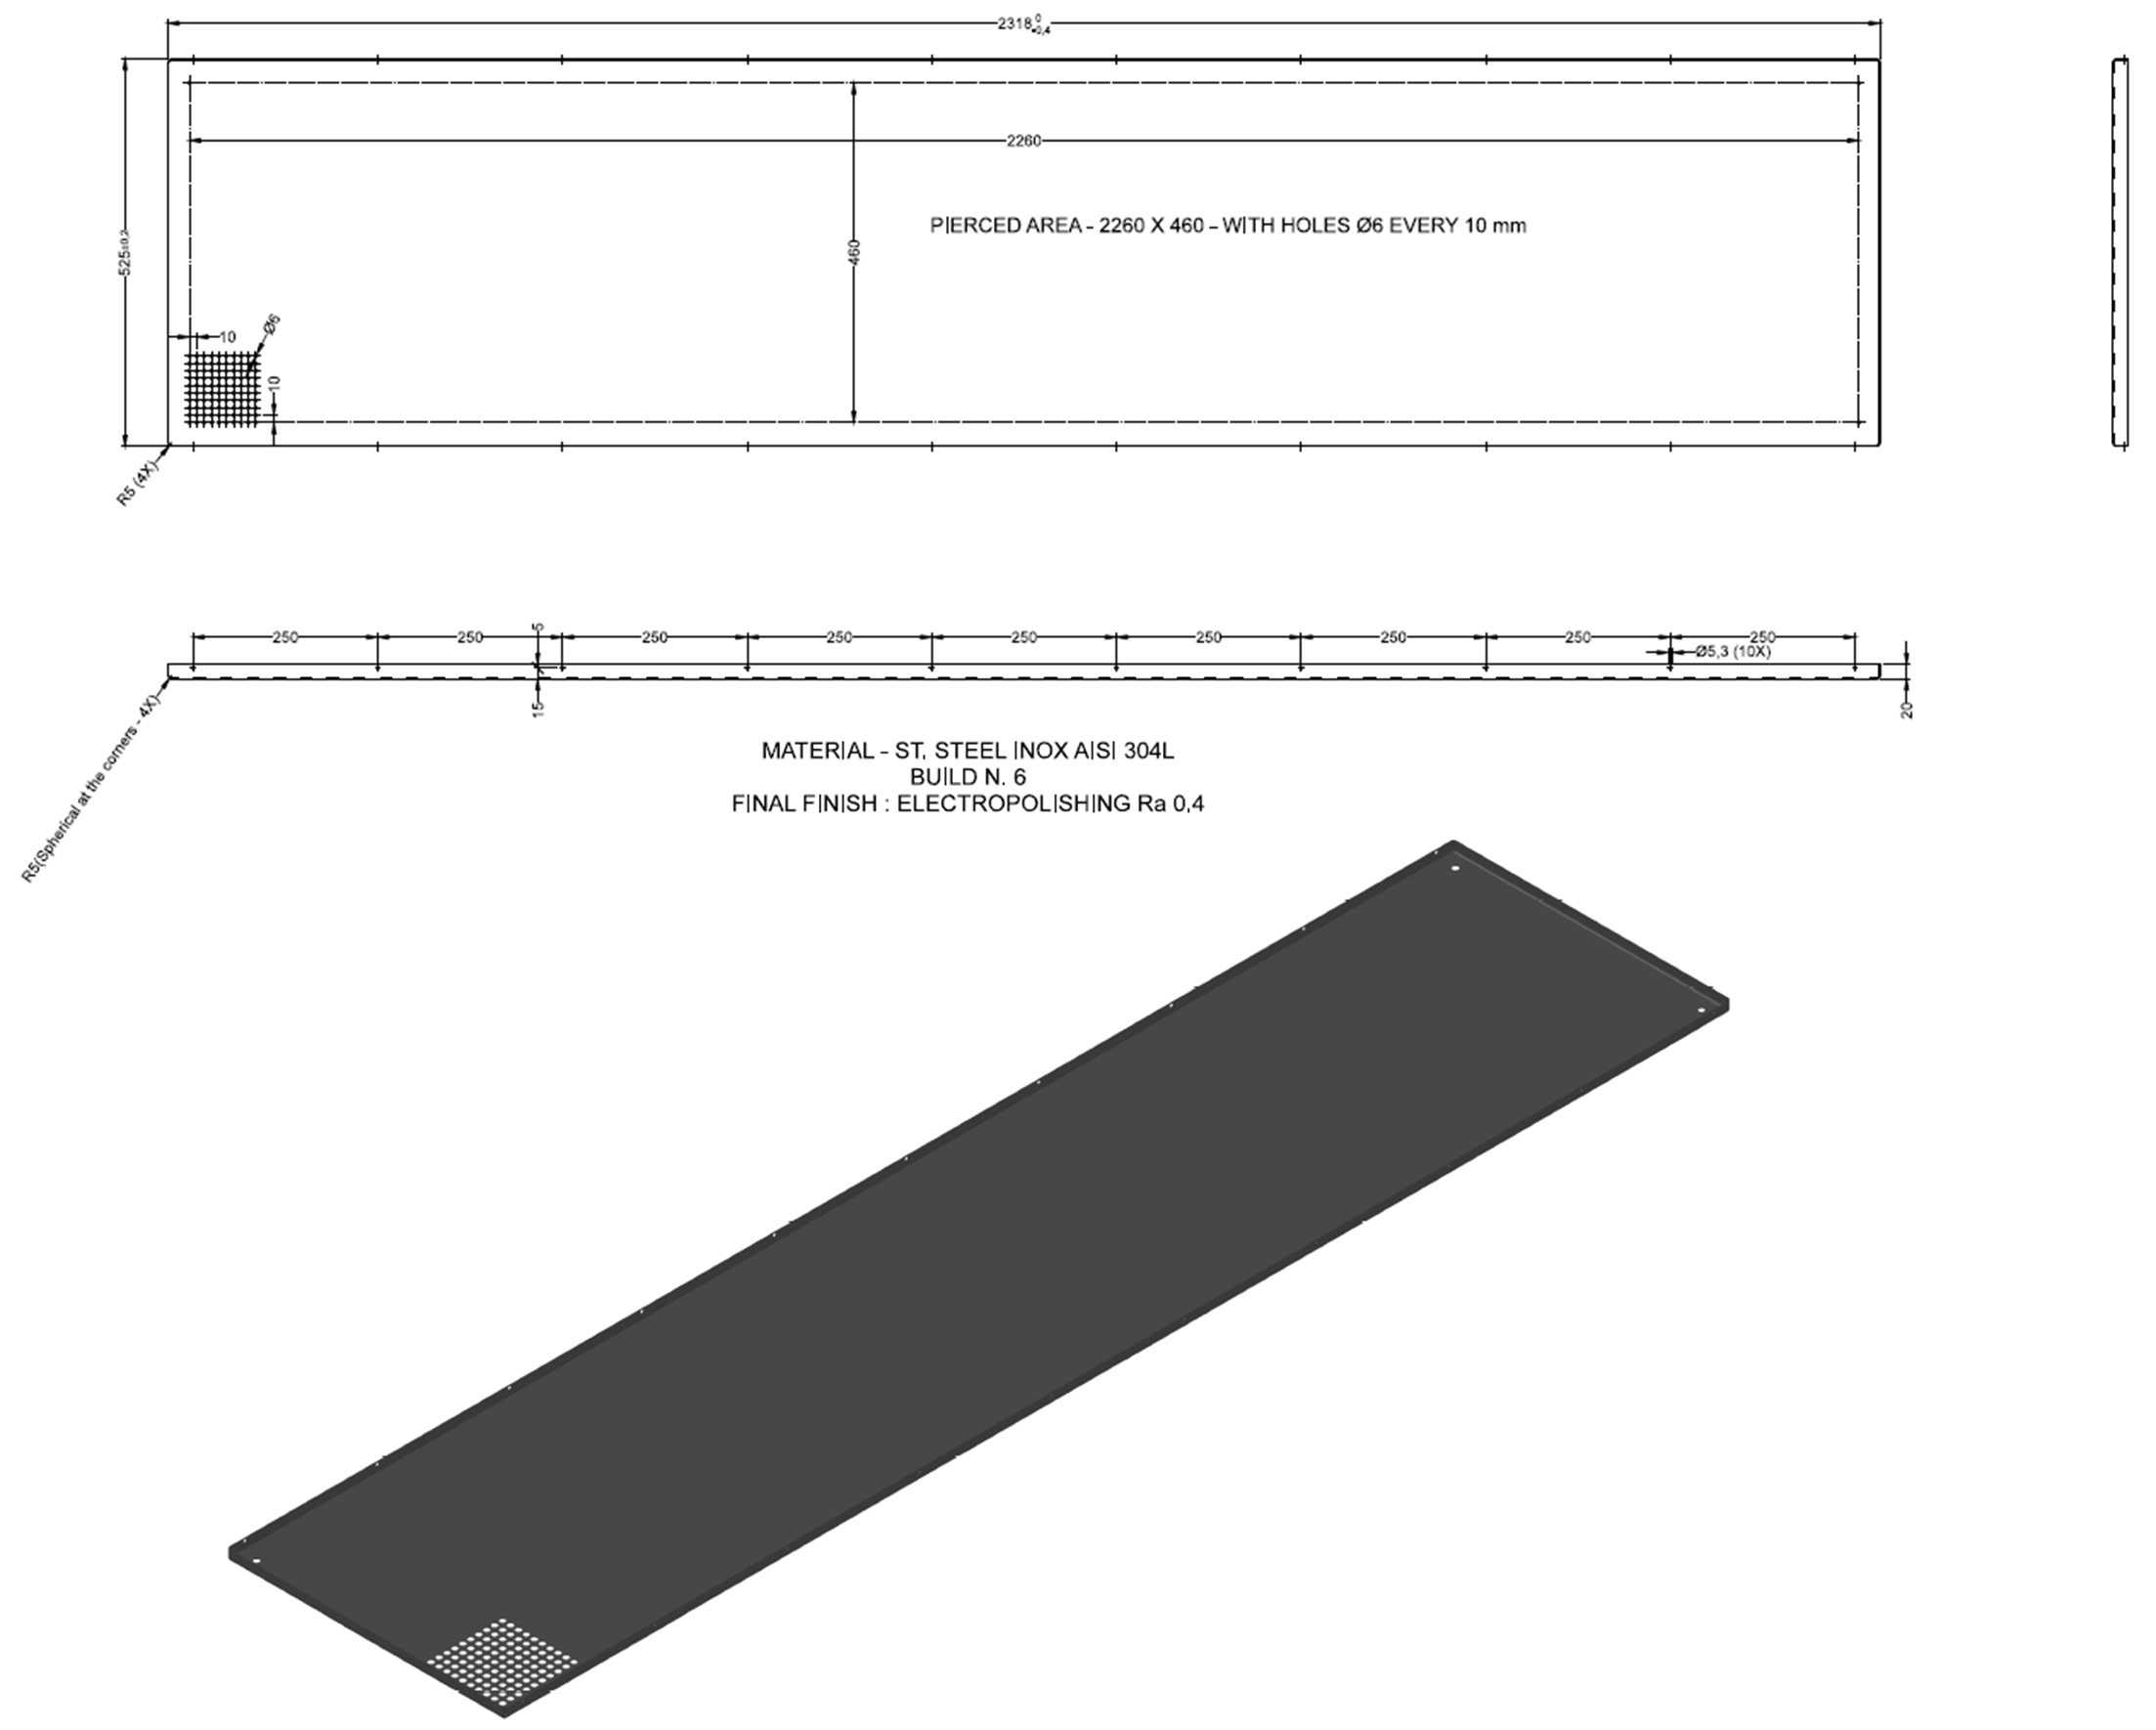
\includegraphics[width=1.0\linewidth]{tpc_fc_gp525x2318piece.png}
\end{cdrfigure}

The choice of electropolished Stainless Steel \textit{AISI 304 L} over Aluminum derives from the experience of the ICARUS detector, moreover:
\begin{itemize}
\item SS and G10 have very similar dilatation coefficients, while Aluminum does not. Choosing SS ensures that all the $GP\,+\,G10$ structure contracts consistently, without too large stresses at the connections; 
\item SS is more ductile than Aluminum, which makes \textit{easier} to machine the corners of the pieces. Note that anyway some imperfections are present even in the SS case, and not all corners will be perfectly identical. 
\item Though Aluminum would guarantee a factor-of-three lighter GP, the overall weight of the SS pieces remains contained (order of 550 kg). \fixme{in other words, SS would also be light enough?}
\end{itemize}

%%%%%%%%%%%%%%%%%%%%%%%%%
\subsection{Field Cage prototype at CERN}
%The main description of the Field Cage Prototype built at CERN, and the tests performed on it, is provided in section ...\fixme{fix}. In here simply the details concerning the GP are reminded. The smaller pieces of GP were installed on the field cage prototype at CERN, to test the configuration. As described elsewhere, the actual distance between the field cage profiles and the GP in this prototype is of 60 mm, therefore a voltage of 60 kV minimum must be attained to verify the ProtoDUNE field configuration. (Figure ~\ref{fig:fc_prot}) During multiple tests in LAr, both with open-air dewars and in a clean liquid configuration, the structure always stood the 60 kV voltage, and it was in general possible to reach the value of 80-100 kV, after which discharges would start. However discharges were always localized on the HV cables, not involving the GP-FC structure.

The main description of the Field Cage Prototype built at CERN, and the tests performed on it, is provided in section ...\fixme{fix}. This section aims to serve as a reminder of the details.
The smaller pieces of the GP were installed on the field cage prototype at CERN to test the configuration. As described elsewhere \fixme{where?} the actual distance between the field cage profiles and the GP in this prototype is of 60~mm, therefore a  minimum voltage of 60~kV must be attained to verify the ProtoDUNE-SP field configuration. (Figure~\ref{fig:fc_prot} \fixme{This figure needs more explanation; what's right and left? where's the 60mm separation?} During multiple tests in LAr, both with open-air dewars \fixme{how do you have LAr in an open dewar?}  and in a clean liquid configuration, the structure consistently withstood the 60 kV voltage, and in fact 80-100 kV was typically achieved, above which discharges would start. The discharges remained localized on the HV cables, and did not involve the GP-FC structure.

\begin{cdrfigure}[CERN Prototype]{fc_prot}{Details of the Field Cage Prototype at CERN, showing the installed GP panels.}
\includegraphics[width=0.8\linewidth]{tpc_fc_prototype.png}
\end{cdrfigure}

%%%%%%%%%%%%%%%%%%%%%%%%%
\subsection{Field Cage and Ground Plane in ProtoDUNE-SP}

The design details of the FC+GP modules for ProtoDUNE is described and shown in the next section. \fixme{add proper reference} Figure~\ref{fig:fc_full} shows a 3D model of one fully assembled module to provide an initial understanding.

\begin{cdrfigure}[CERN Prototype]{fc_full}{3D model of one fully assembled FC+GP module, for the top of the field cage. }
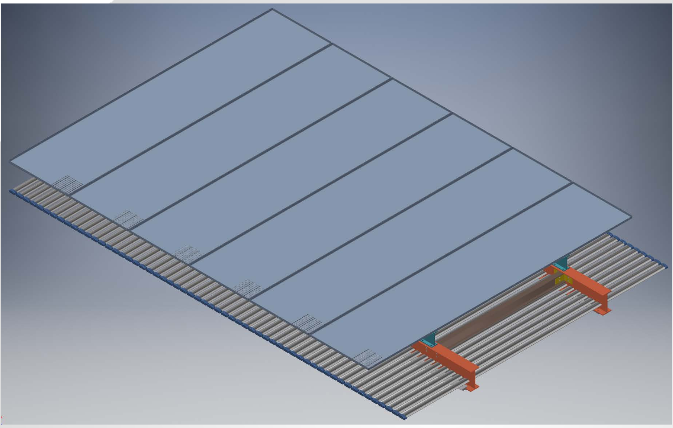
\includegraphics[width=0.8\linewidth]{tpc_topFC.png}
\end{cdrfigure}

One module will be made of six pieces, aligned %put next to each other 
along their long (2318-mm) dimension %direction%: this dimension is made to 
 in order to match the APA and FC module widths. The planes are connected to the FC beam with additional %further 
G10 pieces that are used also to connect adjoining %two neighboring 
GP panels. \fixme{piece vs panel?}

The electrical continuity between consecutive panels can be made %performed 
with metallic screws (with holes on the planes edges) or with looser connections, e.g., copper strips, that better adapt to the shrinking of the structure during cooldown. Copper strips were successfully employed on the CERN FC prototype.
As for most detector systems, the GP should be referenced to the detector ground, located % set 
at the cryostat top.

The GP modules will be installed on the corresponding FC modules in the clean room outside the cryostat, to facilitate the connections. The description of how the top/bottom FC modules are assembled and connected to the CPA before insertion in the cryostat is provided in section ... \fixme{add reference}.

Further GP panels need to be attached to the top FC module:
\begin{itemize}
\item Smaller panels will have to be connected on the modules on one side of the CPA so that, once in position, they %should 
cover the CPA frame. Their dimensions are % is 
still to be defined, depending on the final design of the CPA hanging scheme. Such \fixme{the same pieces are connected, or similar ones are?} pieces should also be connected to the modules covering the opposite drift region, when in final position.
\item An additional % further 
set of small panels should be installed on the outer modules of the FC to extend the GP over the vertical FC walls, which will %to 
further constrain the electric field in these regions. A FEA (Figure ~\ref{fig:fea_overhang}) shows that the optimized overhang distance is 20~cm, provided LAr is at 40~mm above the bottom of the GP. The maximal residual field in this configuration is of the order of 13~kV/cm, with less than 1~kV/cm field in the gas phase.
\end{itemize}

\begin{cdrfigure}[FEA overhang]{fea_overhang}{2D FEA showing the field profile in liquid with a 200-mm overhang, gas-liquid interface 40~mm above the GP bottom. Highest field in the liquid phase is of the order of 13~kV/cm.}
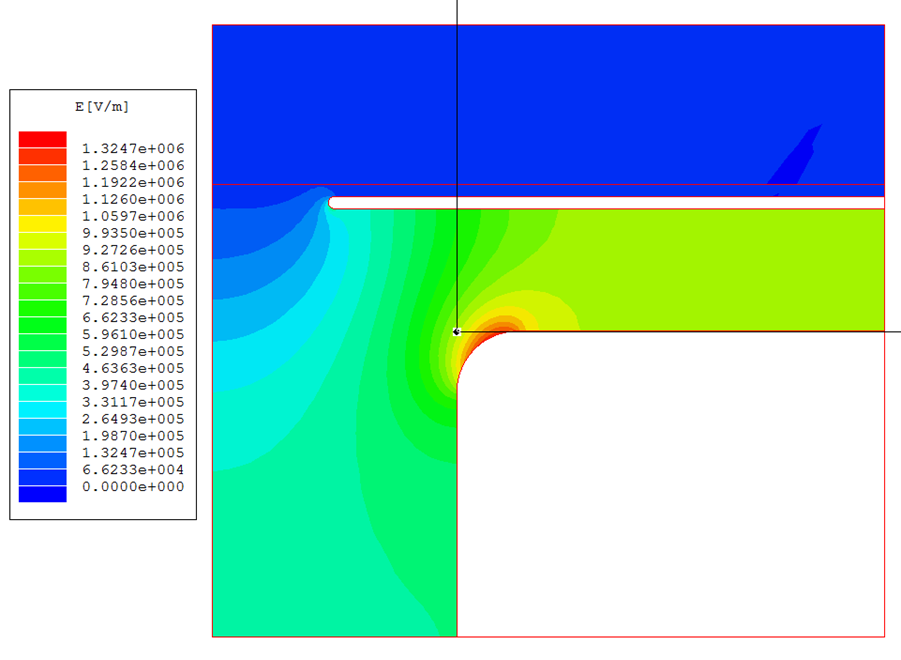
\includegraphics[width=0.7\linewidth]{tpc_fc_gp_overhang.png}
\end{cdrfigure}







%%%%%%%%%%%%%%%%%%%%%%%%%
\subsection{Designs of the Field Cage Modules}

%%%%%%%%%%%%
\subsubsection{Top and bottom modules}


%\begin{cdrfigure}[A top field cage module]{fc-top_module}{A view of a top field cage module}
%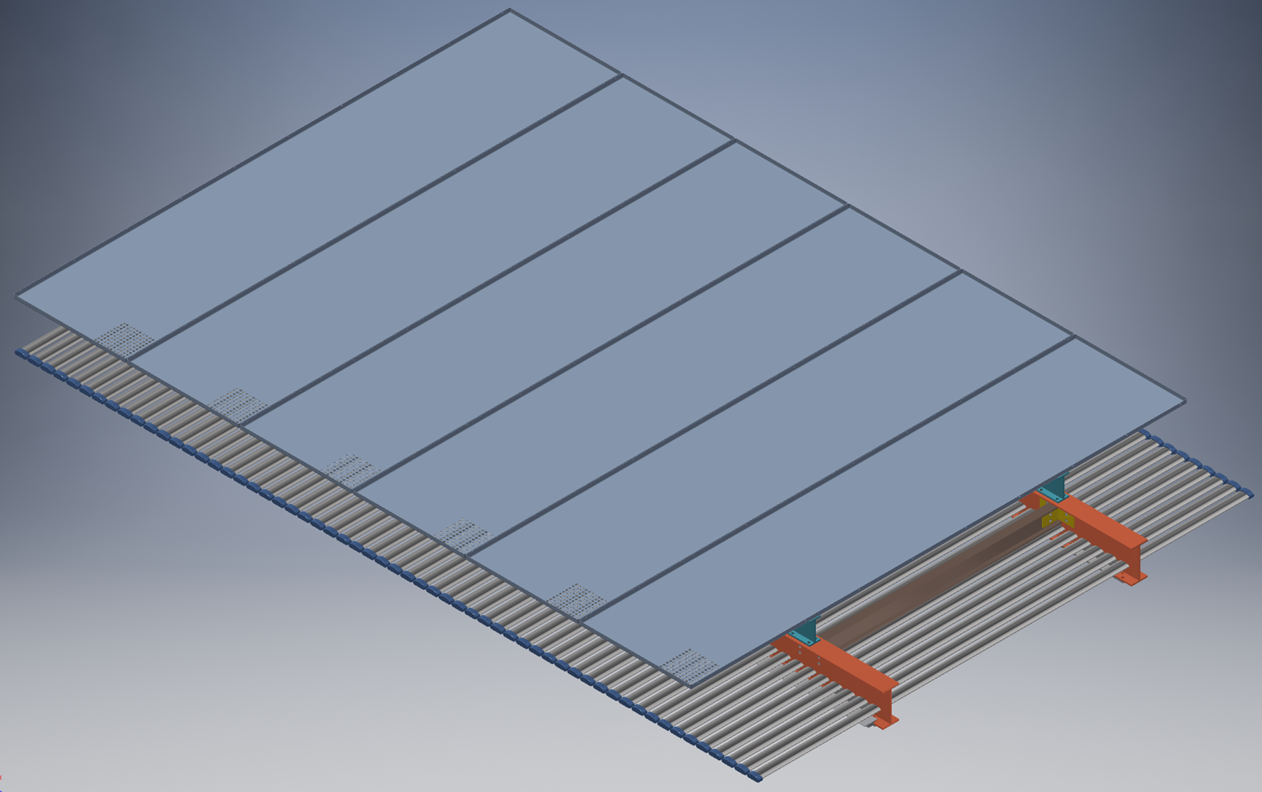
\includegraphics[width=0.8\linewidth]{tpc_fc_top_module.png}
%\end{cdrfigure}


%%%%%%%%%%%%
\subsubsection{End wall modules}

\begin{cdrfigure}[An end wall field cage module]{fc-endwall_module}{A view of an end wall field cage module}
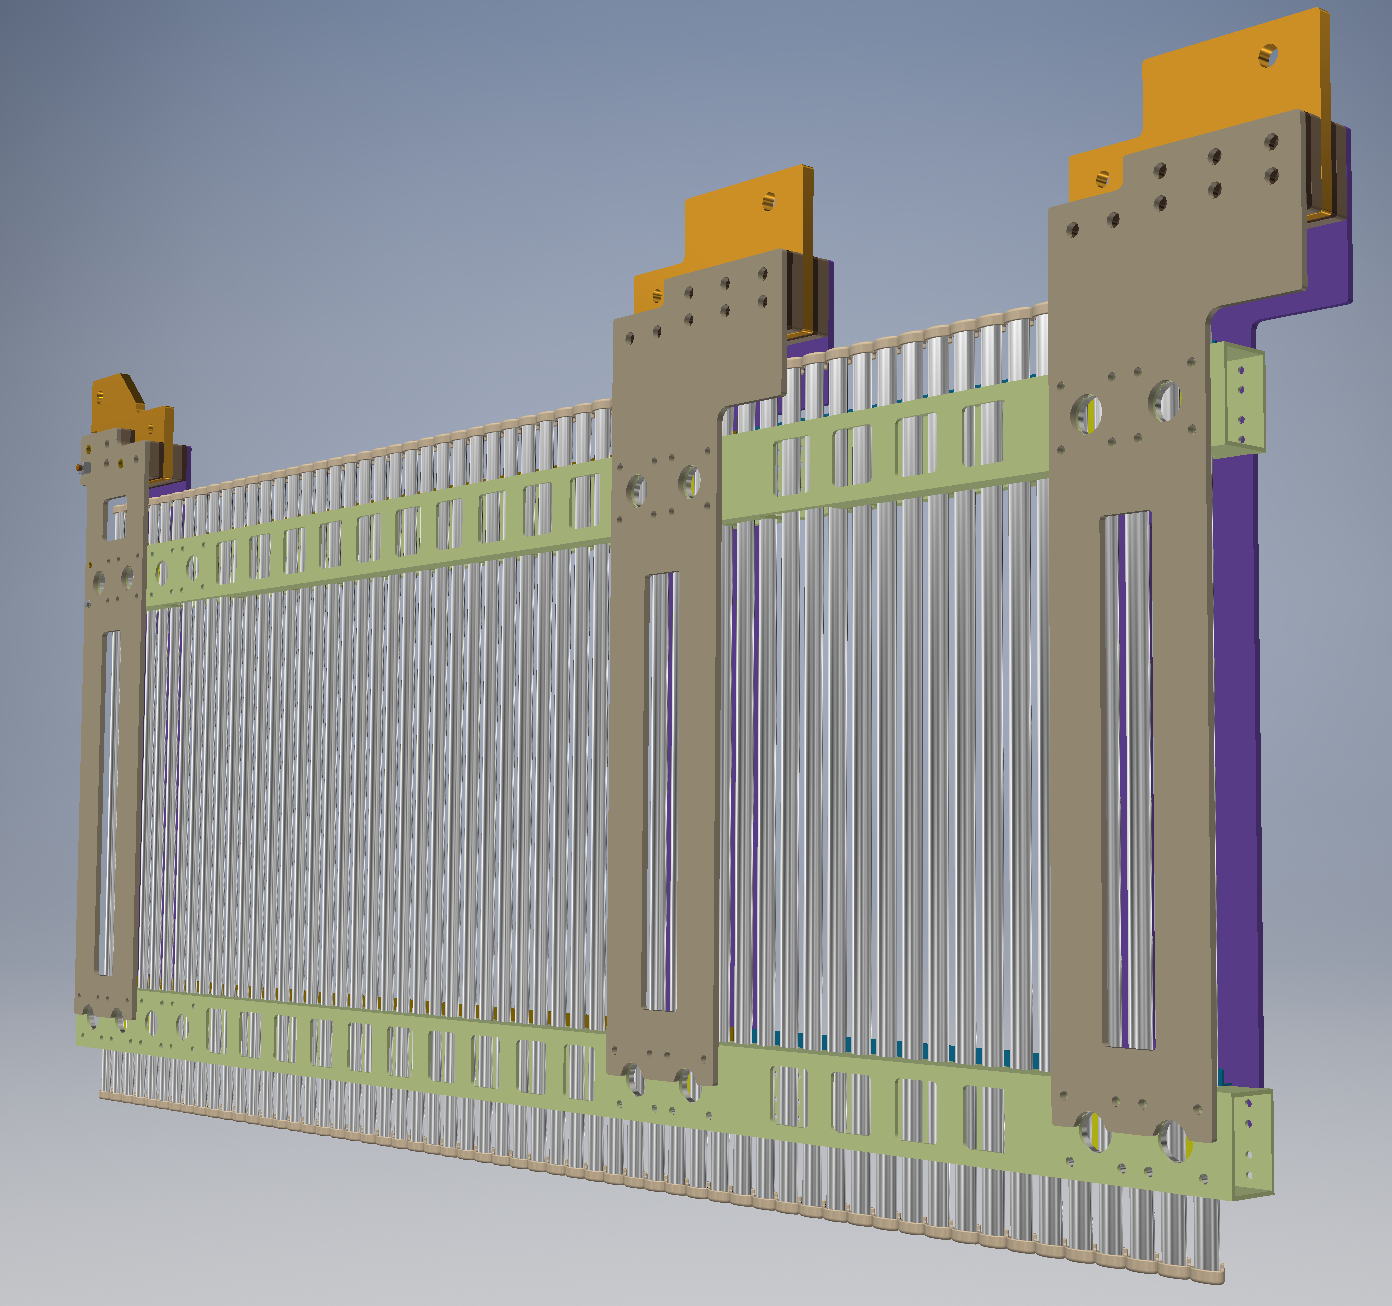
\includegraphics[width=0.8\linewidth]{tpc_fc_endwall_module.png}
\end{cdrfigure}


%%%%%%%%%%%%
\subsection{Interfaces to Other TPC Components}

\subsubsection{Field cage to CPA}

On the top and bottom of the TPC, hinges connect each field cage module to two CPA columns.  This design allows the field cage modules to be pre-attached to the CPAs during installation, and prevents accidental damage to the APA wire plane when raising the field cage module to connect %link 
to the APA.

The end-wall field cage modules are hung from the CPA and APA support rails.  They do not have strong mechanical coupling to the CPAs and APAs, however, at least four resistive divider chains must be connected to the CPA's HV bus.

\begin{cdrfigure}[CPA to field cage connection]{cpa-fc-connection}{A top field cage module connected to two CPA modules}
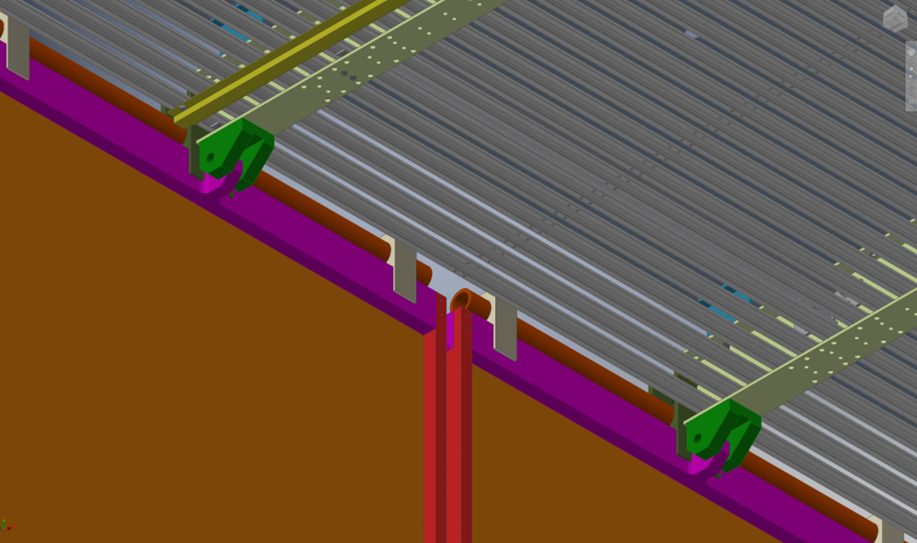
\includegraphics[width=0.8\linewidth]{tpc_fc_cpa_connection.png}
\end{cdrfigure}


%%%%%%%%%%%%
\subsubsection{Field cage to APA}

The I-beams of the top/bottom field cage modules are designed to be latched onto the mating brackets on the APAs.  The design details are currently being developed. % at this moment.  
In addition to the mechanical connection, the ground side of the divider chain must be connected to the APA's frame ground. % as well.


%%%%%%%%%%%%
\subsubsection{Field cage to beam plug}

\fixme{Detail description of the connection between the beam plug and the field cage is described in the beam window section.
}


%%%%%%%%%%%%
\subsubsection{Field cage to calibration lasers}

Four calibration laser windows need to be implemented on the downstream end-wall field cage modules.  The windows are planned to be at the mid-height of the TPC, i.e., at the boundary of two %end-wall field cage 
modules.  The opening for each laser beam is about 15~cm square.  The plan is to shorten three profiles by 7.5~cm from the each edge of the field cage modules.



%%%%%%%%%%%%%%%%%%%%%%%%%
\subsection{QC Procedures}

 


